\subsection{
    Пример для несовместной системы.
}

\begin{example}
    Рассмотрим простейшую систему

    \begin{equation}
        \begin{cases}
            x + y = 0 \\
            x + y = 1
        \end{cases}
    \end{equation}

    двух уравнений с двумя неизвестными. Видно, что эта система несовместна. Последовательно вычисляем

    \begin{equation}
        A = \left(\begin{array}{cc}
            1 & 1 \\
            1 & 1
        \end{array}\right), \thinspace \thinspace
        A^TA = \left(\begin{array}{cc}
            1 & 1 \\
            1 & 1
        \end{array}\right)^2 = \left(\begin{array}{cc}
            2 & 2 \\
            2 & 2
        \end{array}\right), \thinspace \thinspace
        A^Tb = \left(\begin{array}{cc}
            1 & 1 \\
            1 & 1
        \end{array}\right)\left(\begin{array}{c}
            0 \\
            1
        \end{array}\right) = \left(\begin{array}{c}
            1 \\
            1
        \end{array}\right)
    \end{equation}

    Таким образом, нормальная СЛАУ в этом случае состоит из двух одинаковых уравнений:

    \begin{equation}
        \begin{cases}
            2x + 2y = 1 \\
            2x + 2y = 1
        \end{cases}
    \end{equation}

    Множество решений нормальной системы, т.е. множество пар $x, y$, дающих минимальную невязку в исходной системе, на плоскости изображаются прямой $x + y = 0.5$ (рис. \ref{fig:picture_16_1}), а нормальным псевдорешением будет точка этой прямой, ближайшая к началу координат, т.е. точка с координатами $x = 0.25, y = 0.25$. Этой точке соответствует радиус-вектор с наименьшей нормой среди всех радиус-векторов точек прямой $x + y = 0.5$.
    
    К слову, если одно из уравнений исходной системы умножить на коэффициент, то и множество решений нормальной системы, и нормальное псевдорешение данной системы изменятся, так как умножение на коэффициент, вообще говоря, меняет его невязку.

    \begin{figure}[H]
        \centering
        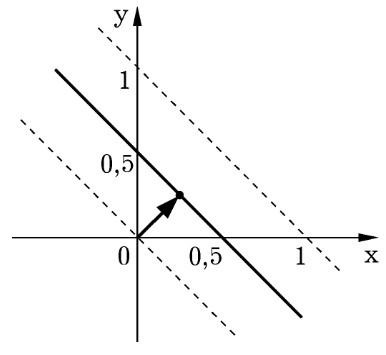
\includegraphics[scale=0.6]{images/module1/question16/1.jpg}
        \caption{}
        \label{fig:picture_16_1}
    \end{figure}

\end{example}
